\documentclass[compress, 13pt, aspectratio=169]{beamer}
\usepackage{siunitx}
\usepackage{physics}
\usepackage{caption}
\usepackage{graphicx}
\usepackage{mhchem}
\usepackage{siunitx}
\usepackage{subfig}
\usepackage{ragged2e}
\usepackage{xcolor}
\usepackage{amsmath, arydshln, array}
\usepackage{setspace}
\usepackage{tikz}
\usepackage{hyperref}
% \usepackage[style=phys, backend=biber, articletitle=false, pageranges=false, citestyle=authoryear]{biblatex}
\usepackage[natbib=true, style=phys, autocite=footnote, articletitle=false, pageranges=false, citestyle=authoryear]{biblatex}
\usepackage{perpage} %the perpage package
\usefonttheme[onlymath]{serif}
\MakePerPage{footnote}
\urlstyle{sf}


% \bibliography{references.bib}
% \usetheme[progressbar=frametitle]{metropolis}
\usetheme{Madrid}
\usecolortheme{default}
\graphicspath{{figures/}}
\addbibresource{reference.bib}

\makeatletter
\newcommand{\srcsize}{\@setfontsize{\srcsize}{5pt}{5pt}}
\makeatother
\setbeamerfont{footnote}{size=\srcsize}
% \renewcommand\footnoterule{}
% \renewcommand{\thempfootnote}{\arabic{footnote}}
% \usepackage[warnundef]{jabbrv}
% \DefineJournalAbbreviation{Test}{Tes}
% \AtEveryCitekey{\iffootnote{\color{red}\scriptsize}{\color{blue}}}
% \DefineJournalAbbreviation{Nuclear Instruments and Methods in Physics Research Section A: Accelerators, Spectrometers, Detectors and Associated Equipment}{Nucl. Instrum. Methods Phys. Res. A}
% \DefineJournalAbbreviation{Instruments}{Instrum.}
% \DefineJournalAbbreviation{Spectrometers,}{Spectro.}

\newcommand{\slfrac}[2]{\left.#1\middle/#2\right.}


\title[Millepede algorithm for Time and Position Calibration of NeuLAND]{Application of Millepede algorithm to Time and Position Calibration of NeuLAND}
\author[Yanzhao Wang]{Yanzhao Wang, Håkan Johansson, Igor Gasparic, and Andreas Zilges}
\institute[University of Cologne $\vert$ AG Zilges $\vert$ ]{Institute for Nuclear Physics, University of Cologne}
\date{\scriptsize HK 51.3 \\DPG-Frühjahrstagung\\Gießen 2024 \\ \vspace{1em} Supported by BMBF (05P21PKFN1)}
\setbeamertemplate{blocks}[rounded][shadow]
\setbeamercolor{footlinecolor1}{fg=white,bg=black}
\setbeamercolor{footlinecolor2}{fg=black,bg=lightgray}
\setbeamertemplate{navigation symbols}{}
% \setbeamertemplate{frametitle}[default][center]

\setbeamertemplate{frametitle}{%
    \vspace{-0.13cm}
\begin{beamercolorbox}[wd=\paperwidth, ht=0.5cm, dp=0.2cm]{frametitle}
\center\usebeamerfont{frametitle}\insertframetitle
\end{beamercolorbox}
}

\renewbibmacro*{name:andothers}{% Based on name:andothers from biblatex.def
  \ifboolexpr{
    test {\ifnumequal{\value{listcount}}{\value{liststop}}}
    and
    test \ifmorenames
  }
    {\ifnumgreater{\value{liststop}}{1}
       {\finalandcomma}
       {}%
     \andothersdelim\bibstring[\emph]{andothers}}
    {}
}

\makeatletter
\setbeamertemplate{footline}
{
  \leavevmode%
  \hbox{%
  \begin{beamercolorbox}[wd=.5\paperwidth,ht=2.25ex,dp=1ex,center]{footlinecolor1}%
    \usebeamerfont{author in head/foot}\insertshortinstitute\insertshortauthor
  \end{beamercolorbox}%
  \begin{beamercolorbox}[wd=.5\paperwidth,ht=2.25ex,dp=1ex,center]{footlinecolor2}%
    \usebeamerfont{title in head/foot}\insertshorttitle\hspace*{2ex}
 \insertframenumber{} / \inserttotalframenumber\hspace*{2ex}
  \end{beamercolorbox}}%
  \vskip0pt%
}
\makeatother
% \setbeamercolor{block body alerted}{bg=alerted text.fg!10}
% \setbeamercolor{block title alerted}{bg=alerted text.fg!20}
% \setbeamercolor{block body}{bg=structure!10}
% \setbeamercolor{block title}{bg=structure!20}
% \setbeamercolor{block body example}{bg=green!10}
% \setbeamercolor{block title example}{bg=green!20}
\begin{document}
{
\usebackgroundtemplate{
\includegraphics[width=\paperwidth]{TitleLogo}}
\begin{frame}
	\titlepage
	\flushright\vspace*{2em}{\tiny Email: \textit{ywang@ikp.uni-koeln.de}}
\end{frame}
}

{
\usebackgroundtemplate{%
	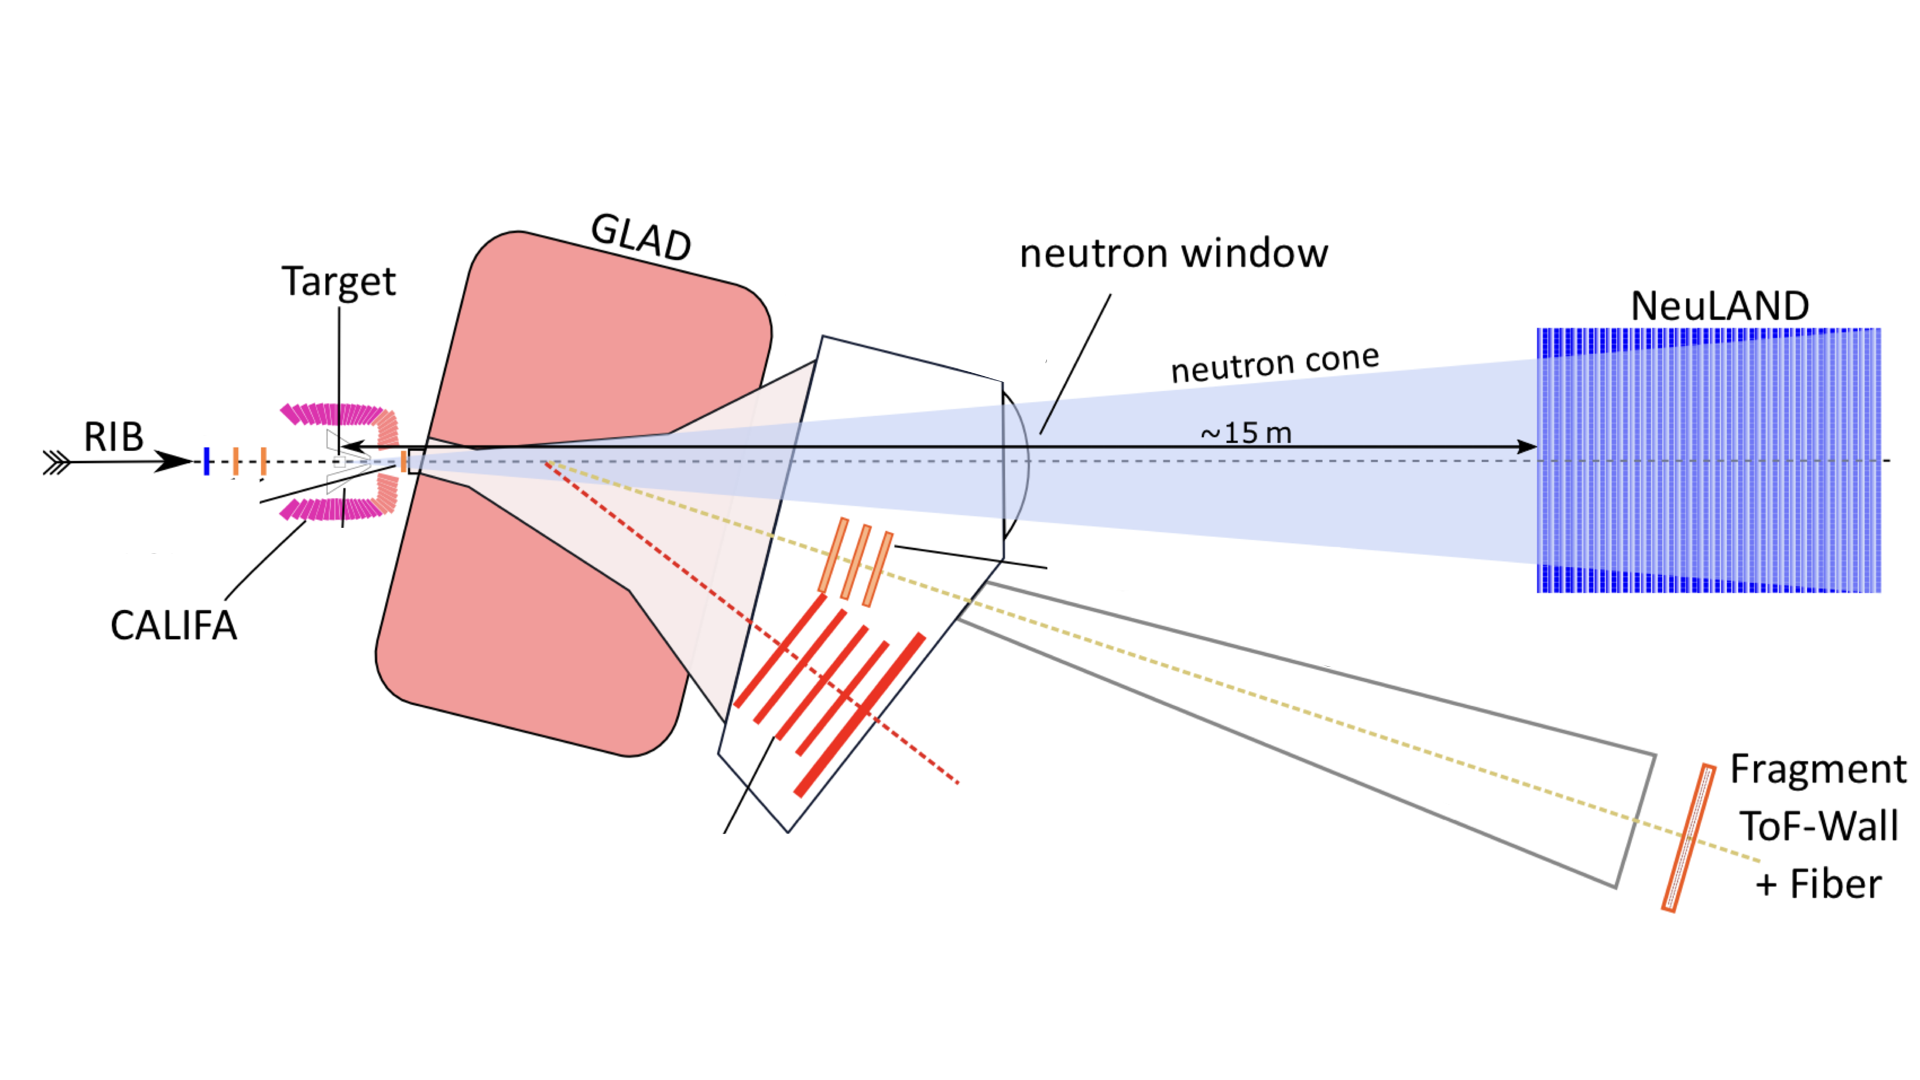
\includegraphics[width=\paperwidth, height=\paperheight]{r3bsetup_empty.png}}
\begin{frame}{NeuLAND setup in $\text{R}^3\text{B}$}

	\begin{columns}[c]
		\begin{column}{0.4\textwidth}
			\pause
			\begin{figure}
				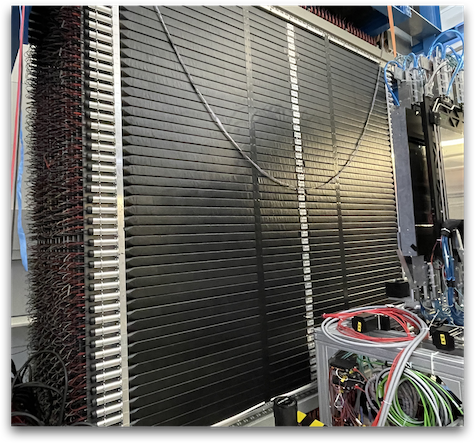
\includegraphics[width = \textwidth]{neulandReal}
			\end{figure}
		\end{column}
		\hspace*{0.5cm}
		\begin{column}{0.3\textwidth}
			\begin{exampleblock}{}
				Geometry:\\
				\begin{itemize}
					\item 26 planes
					\item $\qtyproduct[product-units=power]{250 x 250}{\centi\meter}$
					\item 50 scintillators each plane
					\item 100 PMTs each plane
				\end{itemize}
				\pause
				Measurements:\\
				\begin{itemize}
					% TODO: interaction isn't a good word
					\item \alert<+(1)>{\textbf<.(1)>{interaction position}}
					\item \alert<.(1)>{\textbf<.(1)>{interaction time}}
					\item energy deposition
				\end{itemize}
			\end{exampleblock}
		\end{column}
		\begin{column}{0.3\textwidth}
		\end{column}

	\end{columns}
	\let\thefootnote\relax\footnotetext{\fullcite{BORETZKY2021165701}}
\end{frame}
}

\begin{frame}[t]{Position and time calibration}
	\vspace{-1cm}
	\begin{columns}[t]
		\begin{column}{0.4 \textwidth}
			\vspace*{-0.5cm}
			\begin{figure}[t]
				\hspace*{-0.5cm}
				\centering
				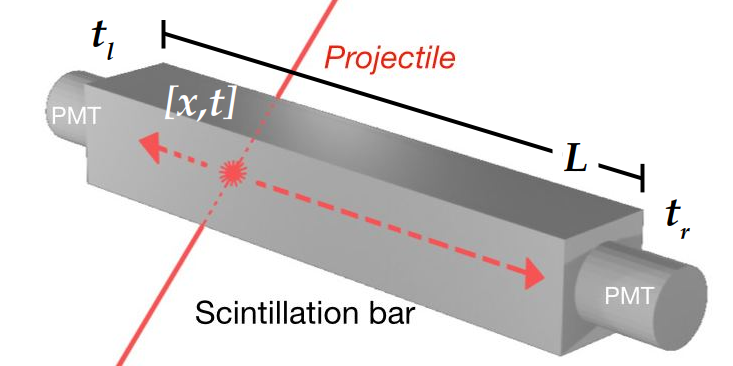
\includegraphics[keepaspectratio, height = 0.4\textheight]{Bar.png}
			\end{figure}
			\vspace{0.5cm}
			\textit{Symbols}:
			\scriptsize{
				\begin{flalign*}
					x           & : \text{position of the interaction } & \\
					t           & : \text{time of the interaction}      & \\
					L           & : \text{length of the scintillator}   & \\
					t_l         & : \text{time of the left PMT signal}  & \\
					t_r         & : \text{time of the right PMT signal} & \\
					\alert{C_e} & : \text{effective speed of light}     & \\
				\end{flalign*}
			}
		\end{column}
		\pause
		\begin{column}{0.48 \textwidth}
			\begin{block}{\small Time relation:}
				$$ t = \frac{t_r + t_l}{2} - \frac{L}{2 \cdot \alert{C_e}} \onslide<+(1)->{+ \alert{t_\text{sync}}}$$
			\end{block}

			\begin{block}{\small Position relation:}
				$$ x = \frac{\alert{C_e}}{2}\left( t_r - t_l \only<+(1)->{ + \alert{t_\text{offset}}} \right)$$
			\end{block}

			\onslide<.->{ \small
				\textit{Additional calibration parameters:}
				\begin{itemize}
					\item \alert{$t_\text{sync}$} : time synchronization among scintillators \\
					\item<+-> \alert{$t_\text{offset}$} : time offset between adjacent PMTs
				\end{itemize}

			}

			\vspace{0.5cm}
			\onslide<+->{
				\textit{Total number of calibration parameters: \alert{\Large{3900}}}
			}
		\end{column}
	\end{columns}
\end{frame}

\begin{frame}[fragile,t]{Calibration principle}
	\vspace*{-2em}
	\begin{columns}[t]
		\begin{column}{0.45 \textwidth}
			\begin{block}{\small Calibration relation}
				$$x = C_1 \cdot t + C_2$$
			\end{block}
			\textit{\footnotesize Data fitting}:
			\begin{columns}
				\begin{column}{0.6 \textwidth}
					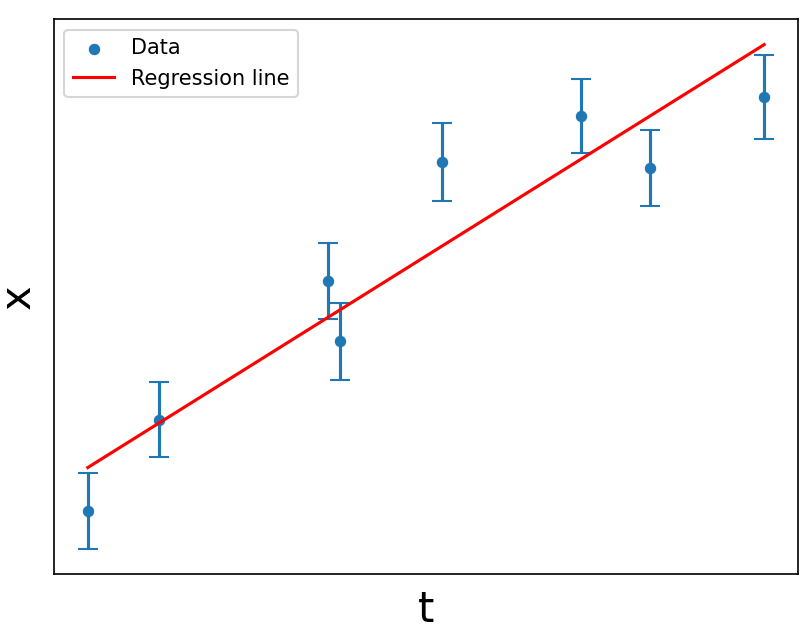
\includegraphics[keepaspectratio, height = 0.4\textheight]{fitting_plot.png}
				\end{column}
				\begin{column}{0.4 \textwidth}
					\small
					\vspace*{-1em}
					\begin{align*}
						 & (t_1,\  x_1) \\
						 & (t_2,\  x_2) \\
						 & \quad ...    \\
						 & (t_i,\  x_i) \\
						 & \quad ...    \\
						 & (t_n,\  x_n)
					\end{align*}
				\end{column}
			\end{columns}
			\vspace{0.3cm}
			\footnotesize{
				\textit{Minimize}
				$$ \text{residual}= \sum_i \frac{(x_i - x(t_i, C_1, C_2))}{ 2* \sigma_i^2} $$
			}
		\end{column}
		\pause
		\begin{column}{0.48 \textwidth}
			\begin{block}{Calibration with muon tracks}
				\vspace*{-1.5em}
				\begin{align}
					\small
					t     & = \slfrac{(t_r + t_l)}{2} - \slfrac{L}{(2 \cdot \alert{C_e})} + \alert{t_\text{sync}} \\
					x     & = \alert{C_e}\cdot \left( t_r - t_l  + \alert{t_\text{offset}} \right) / 2            \\
					x_\mu & = \textcolor{blue}{a^i_x} \cdot z_\mu  + \textcolor{blue}{b^i_x}                      \\
					y_\mu & = \textcolor{blue}{a^i_y} \cdot z_\mu  + \textcolor{blue}{b^i_y}                      \\
					t_\mu & = \textcolor{blue}{a^i_t} \cdot z_\mu  + \textcolor{blue}{b^i_t}
				\end{align}
			\end{block}
			\textit{Calibration parameters for the $i$th event:}
			$$\alert{C_e}, \alert{t_\text{sync}}, \alert{t_\text{offset}}, \textcolor{blue}{a^i_x}, \textcolor{blue}{a^i_y}, \textcolor{blue}{a^i_t}, \textcolor{blue}{b^i_x}, \textcolor{blue}{b^i_y}, \textcolor{blue}{b^i_t}$$
			\pause
			\vspace*{1em}
			\textit{With 10'000 events, the total number of calibration parameters: \alert{\huge 63'900!}}
		\end{column}

	\end{columns}
\end{frame}

\begin{frame}[t]{Current calibration method}
	\vspace*{-2em}
	\begin{columns}[t]
		\begin{column}{0.45 \textwidth}
			\begin{figure}[t]
				\includegraphics<1>[width = \textwidth]{side_view1.png}
				\includegraphics<2>[width = \textwidth]{side_view2.png}
				\includegraphics<3-5>[width = \textwidth]{side_view3.png}
				\includegraphics<6>[width = \textwidth]{side_view4.png}
			\end{figure}
		\end{column}
		\begin{column}{0.45 \textwidth}
			\begin{exampleblock}{\small Procedures}
				\small
				\begin{enumerate}
					\item<1-> Obtain the positions of bars with signals
					\item<2-> Reconstruct the muon track from the bar positions
					\item<3-> Calculate positions of interaction point of the muon
					\item<4-> Obtain calibration parameters via data fitting
				\end{enumerate}
			\end{exampleblock}
			\onslide<5->{
				\textit{\small Data fitting on positions:}\par
				\begin{figure}[t]
					\centering
					\includegraphics[height = 2cm, width = 5cm]{example-image-golden}
				\end{figure}
			}
		\end{column}
	\end{columns}
\end{frame}


\begin{frame}[t,fragile]{Simultaneous fitting of global and local parameters}
	\begin{columns}[t]
		\begin{column}{0.45\textwidth}
			\vspace*{-2em}

			\begin{block}{\small Residual minimization}
				\vspace{-1em}
				$$\large{\partial} \sum^n_{j = 0}\sum_i \frac{\mathcal{Z}^j_i(g_1, ..., g_m, p^j_1, ..., p^j_l)}{ 2 (\sigma^j_i)^2} = 0$$
			\end{block}
			\scriptsize{
				\vspace*{-2.5em}
				\begin{flalign*}
					g_{1\ldots m}   & : \text{$m$ \textit{global parameters}}                          & \\
					p^j_{1\ldots l} & : \text{$l$ \textit{local parameters} for the $j$th $\mu$ track} & \\
					n               & : \text{the total number of $\mu$ tracks}                        &
				\end{flalign*}

				\vspace*{-1em}
			}
			\textit{Newton's method:}

			\vspace*{1em}
			\hspace{3pt}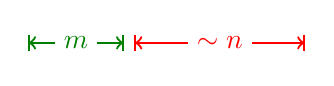
\begin{tikzpicture}[thick]
				\tikzset{good one/.style={color=black!50!green}}
				\draw[good one] (-0.3, 0.1) -- (-0.3, -0.1);
				\draw[<->,good one] (-0.3, 0) -- node[fill=white]{$m$}(0.9, 0);
				\draw[good one] (0.9, 0.1) -- (0.9, -0.1);

				\draw[red] (1.05, 0.1) -- (1.05, -0.1);
				\draw[<->,red] (1.05, 0) -- node[fill=white]{$\sim n$}(3.2, 0);
				\draw[red] (3.2, 0.1) -- (3.2, -0.1);
			\end{tikzpicture}
			\vspace*{-0.9em}
			\setlength\extrarowheight{6pt}
			\scriptsize{
				$$ \left[  \begin{array}{c||c:c:c}
							\sum_j \mathcal{C}_j & \ldots & \mathcal{G}_j & ...    \\[6pt] \hline\hline
							\vdots               & \ddots & 0             & 0      \\[4pt] \hdashline
							\mathcal{G}^T_j      & 0      & \Gamma_j      & 0      \\[6pt] \hdashline
							\vdots               & 0      & 0             & \ddots \\
						\end{array}  \right] \cdot
					\left[ \begin{array}{c}
							\Delta \mathbf{g}   \\[6pt] \hline\hline
							\vdots              \\[4pt] \hdashline
							\Delta \mathbf{p}^j \\[6pt] \hdashline
							\vdots              \\
						\end{array} \right] =
					-\left[ \begin{array}{c}
							\partial_\mathbf{g} \mathcal{Z}     \\[6pt] \hline\hline
							\vdots                              \\[4pt] \hdashline
							\partial_{\mathbf{p}^j} \mathcal{Z} \\[6pt] \hdashline
							\vdots                              \\
						\end{array} \right]
				$$
			}

		\end{column}
		\begin{column}[t]{0.45\textwidth}
			\vspace*{-1em}

			\begin{spacing} {0.5}
				\small
				\textbf{\textit{Matrix Dimension reduction!}} (Schur complement method)
				$$\tilde{\mathcal{C}} \cdot \Delta \mathbf{g} = \mathcal{D}$$
				where
				$$\tilde{\mathcal{C}} = \sum_j \mathcal{C}_j + \sum_j \left(-\mathcal{G}_j \Gamma^{-1}_j \mathcal{G}^T_j \right)$$
			\end{spacing}
			\begin{exampleblock} {Advantages}
				\small
				\begin{itemize}
					\item Simultaneous fitting of all parameters
					\item Computation complexity independent of local parameter size
					\item Direct fitting without any approximation
				\end{itemize}
			\end{exampleblock}
			\textit{Software implementation}: \large{\textbf{Millepede-II}}\footnotemark
			\footnotetext{\fullcite{millepede}}
		\end{column}
	\end{columns}

\end{frame}

\begin{frame}[t]{Comparisons on PMT time offsets}
	\begin{figure}[t]
		\vspace*{-1em}
		\centering
		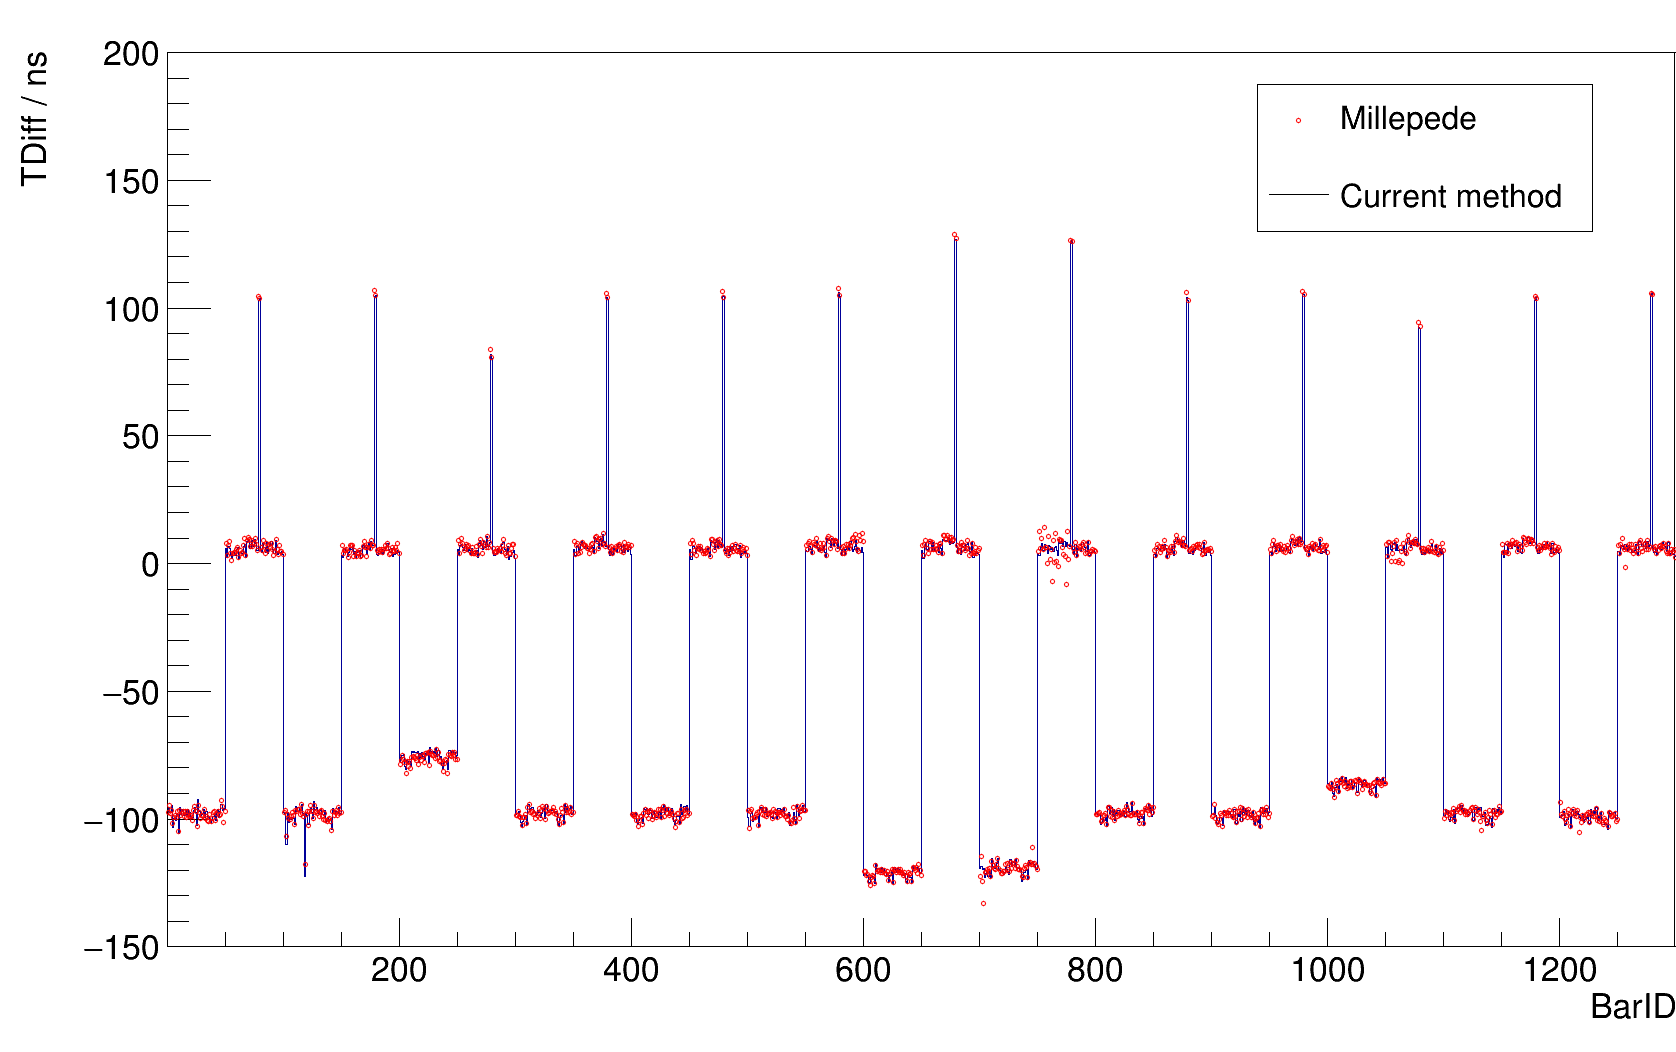
\includegraphics[height = 0.9 \textheight]{t_diff.png}
	\end{figure}
\end{frame}

\begin{frame}[t]{Comparisons on effective speed of light}
	\begin{figure}[t]
		\vspace*{-1em}
		\centering
		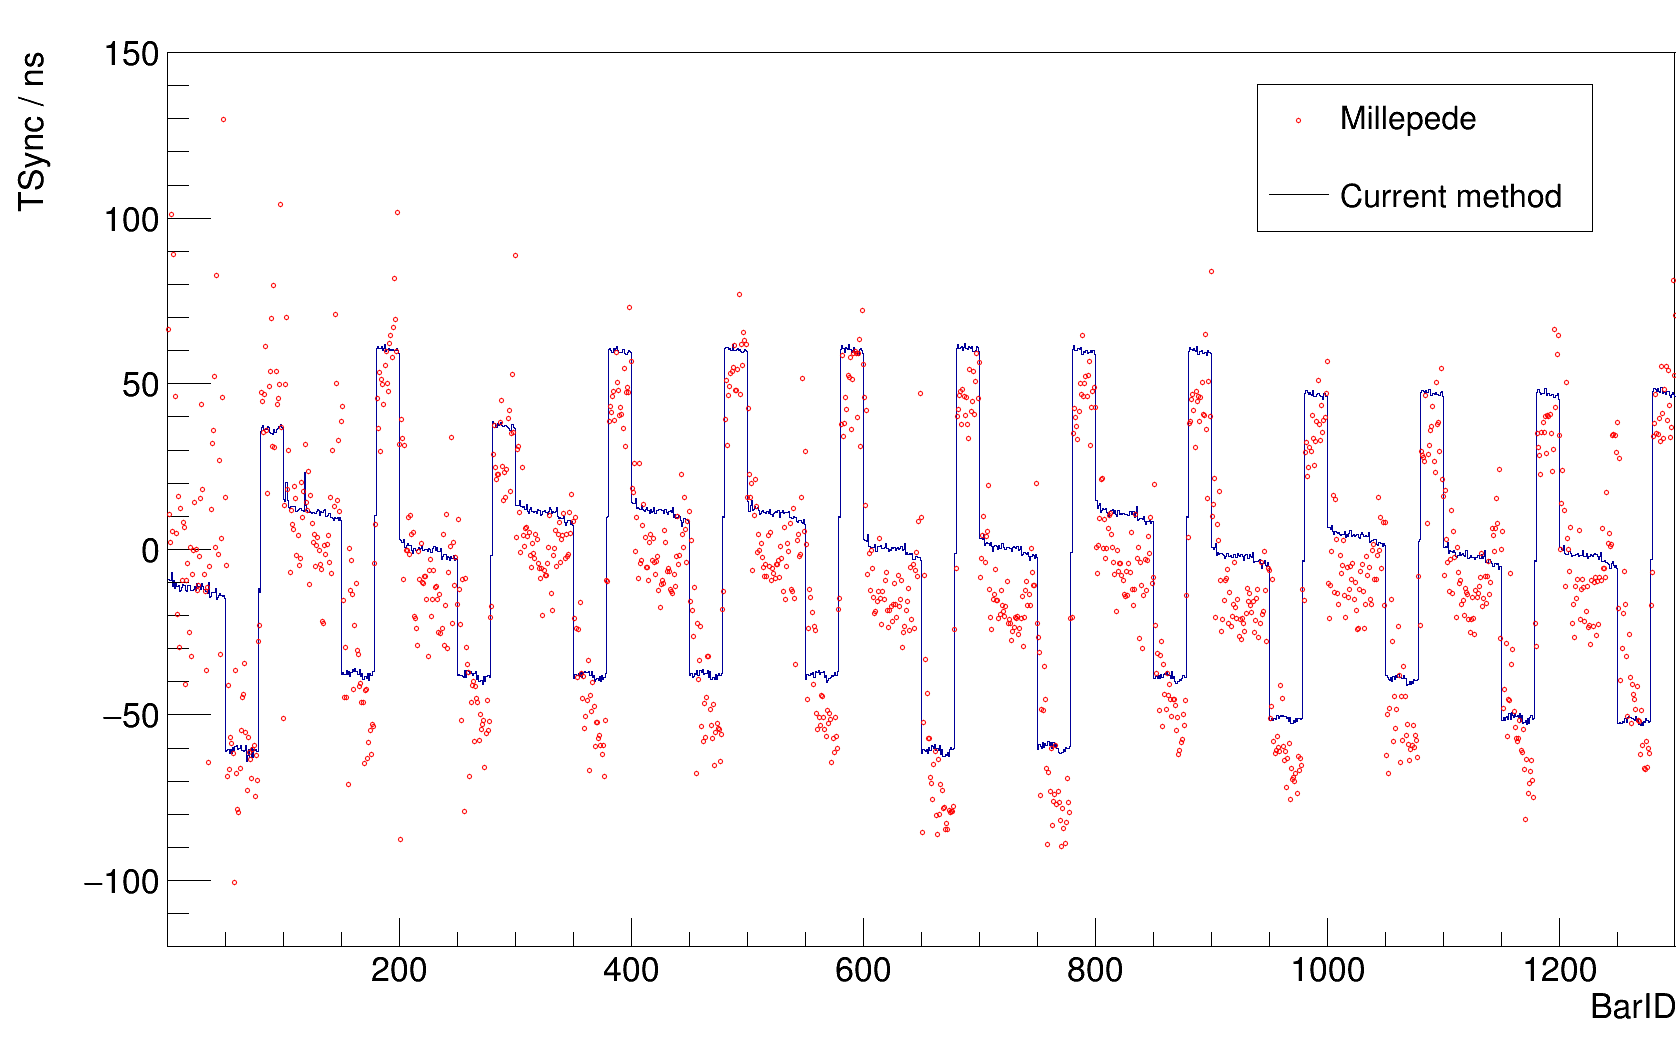
\includegraphics[height = 0.9 \textheight]{tsync.png}
	\end{figure}
\end{frame}

\begin{frame}[t]{Comparisons on time synchronization}
	\begin{figure}[t]
		\vspace*{-1em}
		\centering
		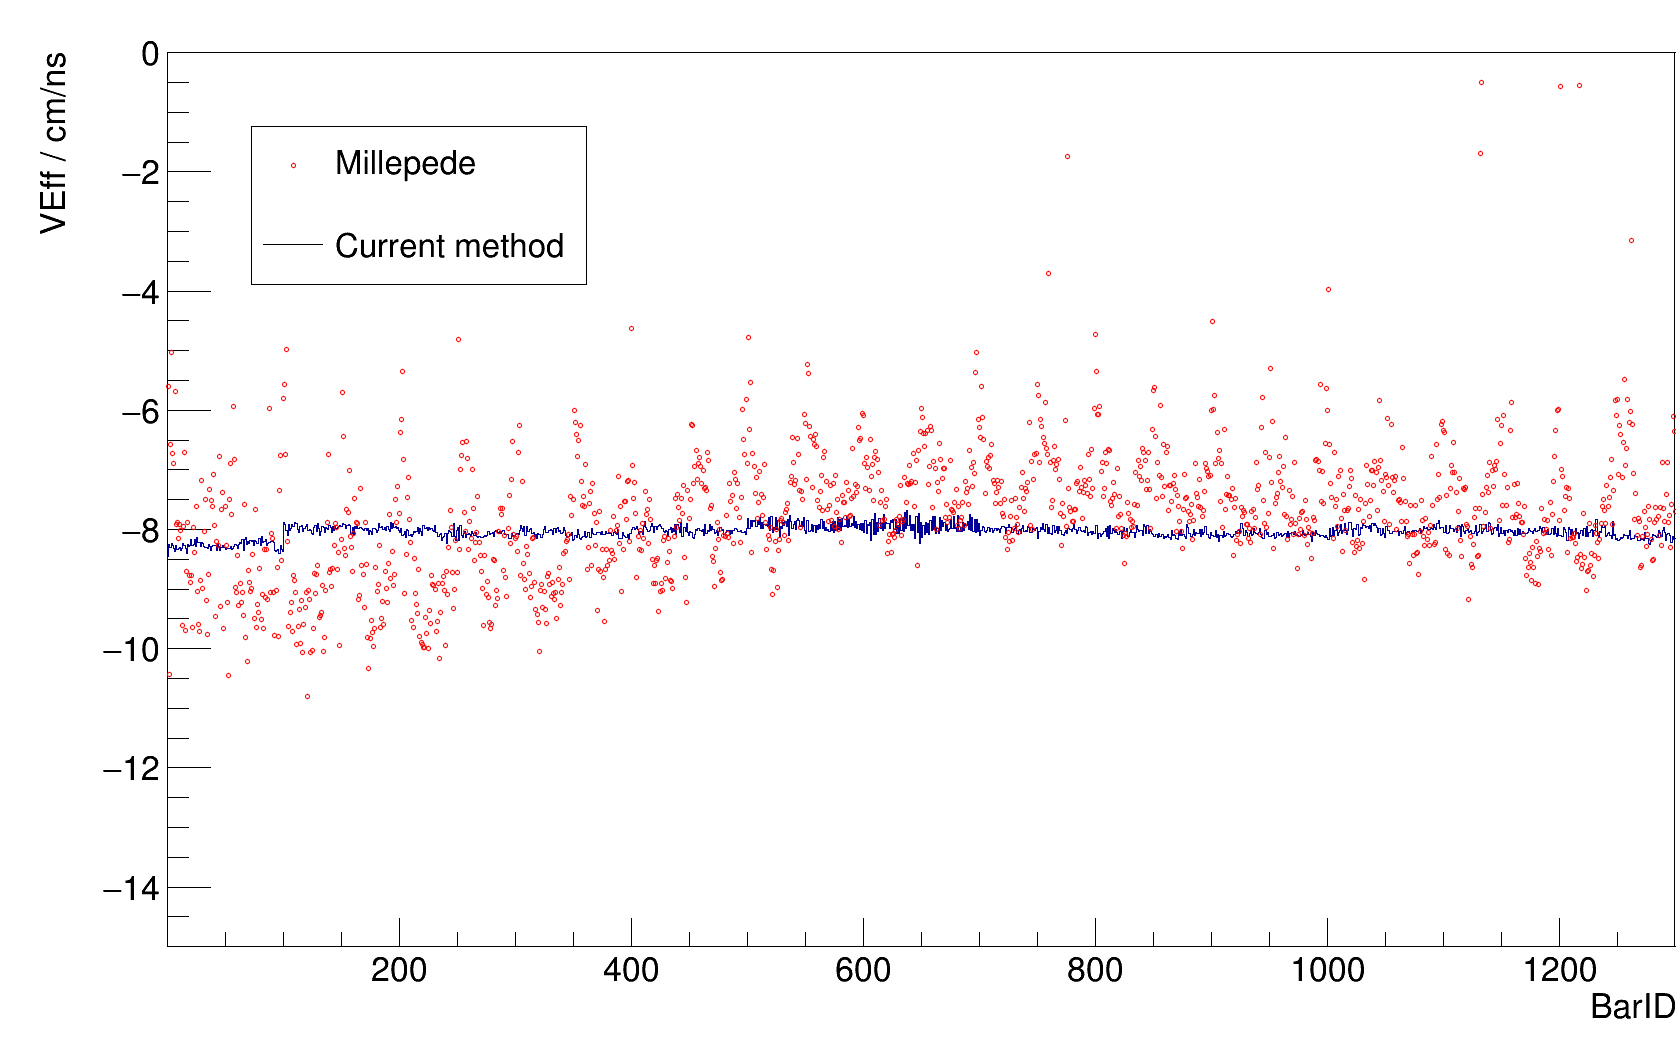
\includegraphics[height = 0.9 \textheight]{effective_c.png}
	\end{figure}
\end{frame}

\begin{frame}[t]{Summary and outlook}

\end{frame}
\end{document}
